\documentclass[10.5pt,a4paper]{article}
\usepackage[margin=2.1cm]{geometry}
\usepackage{booktabs,graphicx,xcolor,enumitem,hyperref,array}
\usepackage{amsmath,amssymb}
\usepackage[T1]{fontenc}
\usepackage{lmodern}
\usepackage{tikz}
\usetikzlibrary{positioning,arrows.meta,fit,backgrounds,calc,shapes.geometric,shadows}
\hypersetup{colorlinks=true,linkcolor=black,urlcolor=blue!50!black}
\setlist{nosep,leftmargin=1.3em}
\setlength{\parskip}{4pt}\setlength{\parindent}{0pt}
\newcommand{\best}[1]{\textbf{#1}}

% ---------- TikZ palette for architecture diagram ----------
\definecolor{ink}{HTML}{2B2D42}
\definecolor{sOneF}{HTML}{E8F1FB}\definecolor{sOneD}{HTML}{3A6EA5}
\definecolor{sTwoF}{HTML}{EAF6EE}\definecolor{sTwoD}{HTML}{3C8D5A}
\definecolor{sThrF}{HTML}{FDF1E6}\definecolor{sThrD}{HTML}{C0662B}
\definecolor{trick}{HTML}{FFF9E3}\definecolor{trickD}{HTML}{B8952E}
\definecolor{ioF}{HTML}{F3F3F6}\definecolor{ioD}{HTML}{6B6F80}
\definecolor{fb}{HTML}{A23B72}

\title{\vspace{-1.2cm}Unified Line$\rightarrow$Word$\rightarrow$Grapheme Cascade for Bangla Handwriting\\[2pt]
\large Executive Summary --- BanglaWriting word-segmentation benchmark}
\date{27 September 2026}
\author{}

\begin{document}
\maketitle
\vspace{-1.4cm}

\section*{Bottom line}
\begin{itemize}
  \item We built \texttt{unified\_cascade/}, one inference engine that runs our Swin-T Mask R-CNN
        line, word and grapheme models as a BN-DRISHTI-style cascade (page $\rightarrow$ lines
        $\rightarrow$ words), with the gains coming from better \emph{inference}.
  \item On the 195 held-out BanglaWriting test pages, the naive cascade scores word F1 0.568.
        \textbf{Benchmark 1} (lines$\rightarrow$words with inference tricks) raises this to
        \best{0.637}, and \textbf{Benchmark 2} (graphemes used to correct words) to \best{0.652}.
  \item With boxes calibrated to BanglaWriting's loose annotation style ($+x$), the same systems
        score 0.765 $\rightarrow$ \best{0.807} $\rightarrow$ \best{0.825}.
  \item BN-DRISHTI, scored with the same metric on the same pages, reaches 0.615. It produces
        1.73 boxes per ground-truth word.
  \item Every threshold and classifier was fit on a separate 65-page dev split, and the test split
        was scored once. The test gains are consistent with the dev gains.
  \item \textbf{Not yet done:} the \emph{single-weight} unified checkpoint is not trained. The results use
        the three existing stage checkpoints behind one engine.
\end{itemize}

\begin{figure}[h]
  \centering
  \includegraphics[width=0.86\linewidth]{test_f1.pdf}
  \vspace{-6pt}
  \caption{Held-out test word F1 (strict one-to-one matching, IoU $\geq$ 0.5). Blue: raw
  predicted boxes. Orange: boxes widened 5\,\% horizontally and 20\,\% vertically (``$+x$'') to match
  BanglaWriting's hand-drawn margins. BN-DRISHTI's boxes are already loose (trained on BN-HTRd), so
  it has no $+x$ variant.}
\end{figure}

\section*{1. Problem and approach}
We started with three independently trained Swin-T Mask R-CNN checkpoints (line, word, grapheme;
144M parameters in total), trained only on synthetic handwriting (syn-hw). BN-DRISHTI, the Bangla state
of practice, runs a YOLOv5 line detector on the page and then a second YOLOv5 word detector on each
line crop.

A literature review (Unified Detector, Hi-SAM, LayoutFormer, CRAFT, Cascade R-CNN/HTC, AutoFocus,
SAHI) found no system that segments line $\supset$ word $\supset$ grapheme instances for a
matra-connected script. We chose a \textbf{cascade with an intelligent inference layer} over a single
one-shot pass, as requested. Each trick is behind a flag so that it can be ablated.

\textbf{Evaluation protocol.}
\begin{itemize}
  \item \textbf{Data:} BanglaWriting, 260 real pages from 260 writers, never used for training.
  \item \textbf{Split:} dev = every 4th page (65 pages, 5{,}387 words); test = the remaining 195 pages
        (15{,}847 words).
  \item \textbf{Metrics:}
    \begin{itemize}
      \item strict one-to-one F1 at IoU 0.5 and 0.75;
      \item Wolf--Jolion split/merge F1;
      \item COCO box AP;
      \item per-error taxonomy: merged / split / loose / missed words, and spurious / partial
            predictions.
    \end{itemize}
\end{itemize}

\section*{2. Benchmark 1 --- lines $\rightarrow$ words (inference tricks)}
Error analysis on the naive cascade showed that most losses came from \emph{how crops are cut and
merged}, not from model capacity. Neighbouring line crops overlap, so words are detected twice or
leak across lines. We tested each fix on dev and kept only those that helped:

\begin{center}\small
\begin{tabular}{p{5.1cm}p{9.6cm}}
\toprule
Trick & Effect on dev (F1@0.5)\\
\midrule
Ownership masking (I1) & Ink closer to a neighbouring line's polygon is faded before word
detection. Best single trick: 0.581 $\rightarrow$ 0.608 (hard, margin 0); the soft variant wins in combination. \\
Duplicate-aware merge (I2) & NMS on intersection-over-smaller-box across line crops. Mostly a
precision gain (P 0.62 $\rightarrow$ 0.69). \\
Mask threshold 0.3, crop pad $\times$0.5 & Fuller word masks and less neighbouring context: +0.03 and
+0.013. \\
Line deskew (I3) & +0.02 alone after a bug fix, neutral once ownership masking is on, so left off. \\
Box convention ($+x$) & Not a detection change: it aligns ink-tight boxes with loose GT. Reported
separately, never instead of raw. \\
\bottomrule
\end{tabular}
\end{center}

Combined, these give \texttt{p1\_best}: dev 0.581 $\rightarrow$ 0.660 and \textbf{test 0.568
$\rightarrow$ 0.637} (+0.069). Precision rises 0.598 $\rightarrow$ 0.708, split/merge F1 0.772
$\rightarrow$ 0.845, and runtime is 0.57\,s/page.

\section*{3. Benchmark 2 --- graphemes to predict words correctly}
After Benchmark 1, the largest error class was \textbf{merged words}: one box covering two or more
ground-truth words, 2{,}103 on test. We tried three designs before one worked.

\begin{enumerate}
  \item \textbf{Rule-based split at grapheme gaps} ($>t\cdot H$). It cut merges by 44\,\%, but
        split errors rose $\approx$7$\times$ and F1 fell to 0.54--0.57. A pixel gap alone cannot tell
        intra-word from inter-word spacing.
  \item \textbf{Learned gap arbitration with re-boxing.} Every gap between grapheme runs is
        classified from word-model, grapheme and ink features. Gap AUC reached 0.98, yet word F1
        was only 0.58. Diagnosis: re-boxing \emph{every} word from its graphemes alone lost 0.10 F1.
  \item \textbf{Conservative edits (deployed).} The word model's boxes are kept, and graphemes only
        \emph{split} a word where the classifier is confident ($P>0.5$). A separate
        \textbf{punctuation} classifier adds or detaches marks (dari, comma, dash), which BanglaWriting labels as words. With no edits, the output is bit-identical to
        Benchmark 1, so every change is attributable to grapheme evidence.
\end{enumerate}

\textbf{What the graphemes contribute} (page-grouped 5-fold cross-validation on dev):
\begin{itemize}
  \item Gap AUC rises 0.932 with the word-model boundary alone $\rightarrow$ 0.965 with grapheme gap
        features $\rightarrow$ 0.970 with ink/matra-crossing features $\rightarrow$ 0.981 with an MLP.
  \item The matra (headline stroke), which joins graphemes \emph{within} a word, is a useful,
        script-specific signal.
\end{itemize}

\begin{center}\small
\begin{tabular}{lcccccc}
\toprule
Test split (195 pages) & F1@0.5 & F1@0.5 $+x$ & SM-F1 $+x$ & AP50 $+x$ & merged & missed\\
\midrule
Benchmark 1 (\texttt{p1\_best}) & 0.637 & 0.807 & 0.866 & 0.707 & 2103 & 1919\\
+ grapheme split (\texttt{g\_learned}) & 0.650 & 0.820 & 0.872 & 0.723 & 1613 & 1926\\
+ punctuation (\texttt{g\_v3}, Benchmark 2) & \best{0.652} & \best{0.825} & \best{0.877} & \best{0.735} & \best{1478} & \best{1694}\\
\bottomrule
\end{tabular}
\end{center}

On test, graphemes reduce merged-word errors by \textbf{30\,\%} (2{,}103 $\rightarrow$ 1{,}478) and
missed words by 12\,\%. F1 improves +0.015 raw and +0.017 with $+x$, at a cost of about 1.05\,s/page
extra (1.62 vs 0.57\,s/page).

\section*{4. Full results (held-out test)}
\begin{center}\small
\begin{tabular}{lccccccc}
\toprule
System & F1@.5 & P & R & F1@.75 & SM-F1 & AP50 & s/page\\
\midrule
BN-DRISHTI (YOLOv5 line$\rightarrow$word) & 0.615 & 0.485 & 0.841 & 0.219 & 0.674 & 0.582 & --- \\
Naive Swin cascade & 0.568 & 0.598 & 0.541 & 0.058 & 0.772 & 0.356 & 0.47\\
Naive Swin cascade $+x$ & 0.765 & 0.806 & 0.729 & 0.458 & 0.824 & 0.665 & 0.47\\
Benchmark 1 & 0.637 & 0.708 & 0.580 & 0.099 & 0.845 & 0.436 & 0.57\\
Benchmark 1 $+x$ & 0.807 & 0.897 & 0.734 & 0.495 & 0.866 & 0.707 & 0.57\\
Benchmark 2 & 0.652 & 0.695 & 0.614 & 0.100 & 0.838 & 0.459 & 1.62\\
Benchmark 2 $+x$ & \best{0.825} & 0.879 & \best{0.777} & 0.495 & \best{0.877} & \best{0.735} & 1.62\\
\bottomrule
\end{tabular}
\end{center}

\textbf{How to read these numbers.}
\begin{itemize}
  \item Our raw F1@0.75 is low because our boxes hug the ink while BanglaWriting's boxes include
        margin. This is an annotation-convention gap, and $+x$ recovers it (0.10 $\rightarrow$ 0.50).
  \item BN-DRISHTI's recall is high because it emits many overlapping boxes. Its precision is 0.485.
\end{itemize}

\section*{5. Quality assurance}
Sonnet agents wrote the code, and independent Opus agents reviewed it before any number was
trusted. The reviews found and fixed four bugs:
\begin{enumerate}
  \item Deskew left the rotated crop uncut, which shrank text under the strip-height cap (deskew
        went from $-0.036$ to $+0.02$).
  \item The ownership mask was misaligned by up to 3\,px.
  \item The punctuation step merged whole lines into one ``mark''.
  \item A missing configuration would have crashed the test run.
\end{enumerate}
The reviews also confirmed:
\begin{itemize}
  \item there is no ground-truth use at inference;
  \item training and inference features match (live-vs-cached parity within 0.9\,px);
  \item the out-of-fold results match in-sample ones (0.670 vs 0.670), and nested CV costs
        $\leq$0.001.
\end{itemize}

\section*{6. Remaining headroom and recommendations}
Oracle analysis on dev ($+x$ F1, current 0.812--0.815) shows where the next gains are:
\begin{itemize}
  \item \textbf{Punctuation} (oracle +0.05, captured +0.003). The classifier is weak (AUC 0.83;
        651 positives out of 15.6k candidates). A dedicated small-mark detector trained on
        synthetic punctuation is the top recommendation.
  \item \textbf{Box geometry of split words} (oracle +0.05). Correct splits with GT-quality boxes
        would reach 0.905, against 0.851 with our current box geometry.
  \item \textbf{Split candidates.} 104 merged words have no grapheme gap at the true boundary, so
        split recall is capped by candidate generation.
  \item \textbf{Single-weight model.} Train \texttt{composite/} (shared backbone, three heads,
        $-42$\,\% parameters) with cascade-aware sampling. An estimated $\sim$1 GPU-week; the engine
        is model-agnostic and will run on it unchanged.
  \item \textbf{Speed.} The grapheme pass triples runtime. It could run only on words the
        classifier flags as likely merges, since most words need no grapheme evidence.
\end{itemize}

\newpage
\section*{7. Detailed System Architecture and Workflow}

The system takes a single page image and produces word-level boxes in three cascaded stages, each handled by an independently trained Swin-T Mask R-CNN checkpoint (line, word, grapheme; 144M parameters combined, all trained only on synthetic handwriting). \texttt{unified\_cascade/engine.py} runs the three models as one pipeline rather than three separate scripts, so every inference trick below is a shared, ablatable stage between them.

\textbf{Stage 1: line detection.} The page image is passed whole to the line-level Swin-T Mask R-CNN, which returns one polygon mask per handwritten line, plus a detection confidence score. These polygons are the only ground truth the rest of the pipeline sees; there is no oracle information used anywhere at inference time (confirmed by independent review, Section 5).

\textbf{Stage 2: word detection with cascade inference tricks.} Each line polygon defines a crop of the page, padded outward (\texttt{cascade.crop\_box}, \texttt{STAGE\_PADS}) so that ascenders, descenders, and slightly rotated ink are not clipped. Because neighbouring lines are close together and their padded crops overlap, two problems appear: (a) ink belonging to line $N$ bleeds into the crop for line $N+1$, so the word detector sometimes detects a ``word'' that is really a fragment of the line above or below it, and (b) a word sitting in the overlap band gets detected twice, once in each line's crop, producing duplicate boxes. The naive cascade that does nothing about this scores test F1 0.568.

Two mechanisms address this directly. Ownership masking (I1) precomputes a per-pixel distance field over the page (\texttt{ownership\_map}, at 4$\times$ downsampling) recording, for every pixel, how much closer it is to its own line's polygon than to any neighbour's. When a line's crop is built, pixels that are closer to a neighbouring line by more than a margin (0.25 $\times$ that line's own line-height) are suppressed before the word detector ever sees them. ``Hard'' ownership paints those pixels white outright (dev F1 0.581 to 0.608 on its own, the single best trick); ``soft'' ownership fades them gradually instead of a binary cut, which loses less real ink near the boundary and is the variant that wins once combined with the other tricks. Duplicate-aware merge (I2) then removes the remaining cross-crop duplicates with greedy NMS, but measured as intersection-over-smaller-box-area rather than standard IoU: because the same physical word can come out as a tight box from one crop and a slightly larger, context-bleeding box from the neighbouring crop, ordinary IoU (intersection over union) underestimates the overlap when the two box sizes differ, and duplicates survive. Intersection-over-smaller-box (threshold 0.6) catches this regardless of size skew and is mostly a precision fix (P 0.62 to 0.69 on dev). Two smaller knobs round out Benchmark 1: lowering the mask threshold from the default 0.5 to 0.3 keeps more of the soft edge of the predicted mask, giving fuller word boundaries (+0.03 F1); shrinking the crop padding to 0.5$\times$ pulls in less neighbouring-line context to begin with (+0.013 F1). Line deskew (rotating the crop to the line's centerline angle before detection) helps in isolation (+0.02) but is redundant once ownership masking is active, so it is left off in the deployed configuration. Combined, these four tricks are Benchmark 1 (\texttt{p1\_best}): test F1 0.568 to 0.637, precision 0.598 to 0.708, split/merge F1 0.772 to 0.845, at 0.57\,s/page.

\textbf{Stage 3: grapheme detection and word correction.} A third Swin-T Mask R-CNN detects graphemes (Bangla akkhor units) inside each line crop. These are not reported as output; they exist purely as evidence to correct Stage 2's word boxes. The key script, \texttt{gaps.py}, groups a word's own grapheme detections into runs and asks, for every gap between two runs, whether that gap is inside one word (should stay merged) or between two words (should be split). The decisive script-specific feature is the matra: the horizontal headline stroke that visually joins graphemes within a single Bangla word. A grapheme gap crossed by a continuous matra is almost always intra-word; a gap with no matra crossing it is much more likely to be a true word boundary. This ``\texttt{matra\_crossing\_frac}'' feature, combined with ink density in the gap and the gap's size relative to the line height and the median gap in that line, feeds a small MLP gap classifier whose out-of-fold AUC rises from 0.932 (word-model boundary alone) to 0.965 (adding grapheme-run gap geometry) to 0.970 (adding ink/matra features) to 0.981 (the full MLP).

Two earlier designs used this classifier more aggressively and both regressed F1 despite the strong AUC: a pure pixel-gap rule cut merged-word errors by 44\% but multiplied split errors roughly sevenfold (F1 fell to 0.54--0.57), and re-boxing every word from its grapheme runs (rather than only editing) lost 0.10 F1 even with a 0.981-AUC classifier, because re-boxing damages words the classifier is uncertain about just as often as it fixes ones it is confident about. The deployed design is conservative: the word model's box is the default, and graphemes are only allowed to split a word where the classifier's confidence exceeds $P>0.5$. Below that threshold nothing changes. This makes the correction strictly additive rather than substitutive: with the classifier disabled, Benchmark 2's output is bit-identical to Benchmark 1, so every change in the final numbers is directly attributable to grapheme evidence, not to noise from re-detection.

A parallel path in \texttt{punct.py} handles punctuation (dari, comma, dash), which BanglaWriting's annotators label as their own word-level boxes. Small connected components near a word's edge that are punctuation-sized (not a whole word's or line's worth of ink) are scored by a lightweight classifier and either split off from the word they are currently glued to (\texttt{punct\_detach}) or instantiated as a new mark box (\texttt{punct\_new}).

\textbf{Output:} the final prediction is a set of word polygons/boxes, each carrying the word detector's confidence score (or, where a split fired, the scores of the resulting pieces), plus any separated punctuation marks. On test, these two grapheme-driven corrections together cut merged-word errors 30\% (2{,}103 to 1{,}478) and missed words 12\% (1{,}919 to 1{,}694), raising F1 0.637 to 0.652 raw (0.807 to 0.825 with $+x$ calibration), at a cost of roughly 1.05 extra seconds per page (0.57 to 1.62\,s/page) for the added grapheme pass.

\section*{8. Detailed System Architecture Diagram}

Figure \ref{fig:architecture} shows the end-to-end cascade pipeline. The architecture consists of three distinct stages, each operating on progressively finer units:

\begin{figure}[h]
\centering
\resizebox{\linewidth}{!}{%
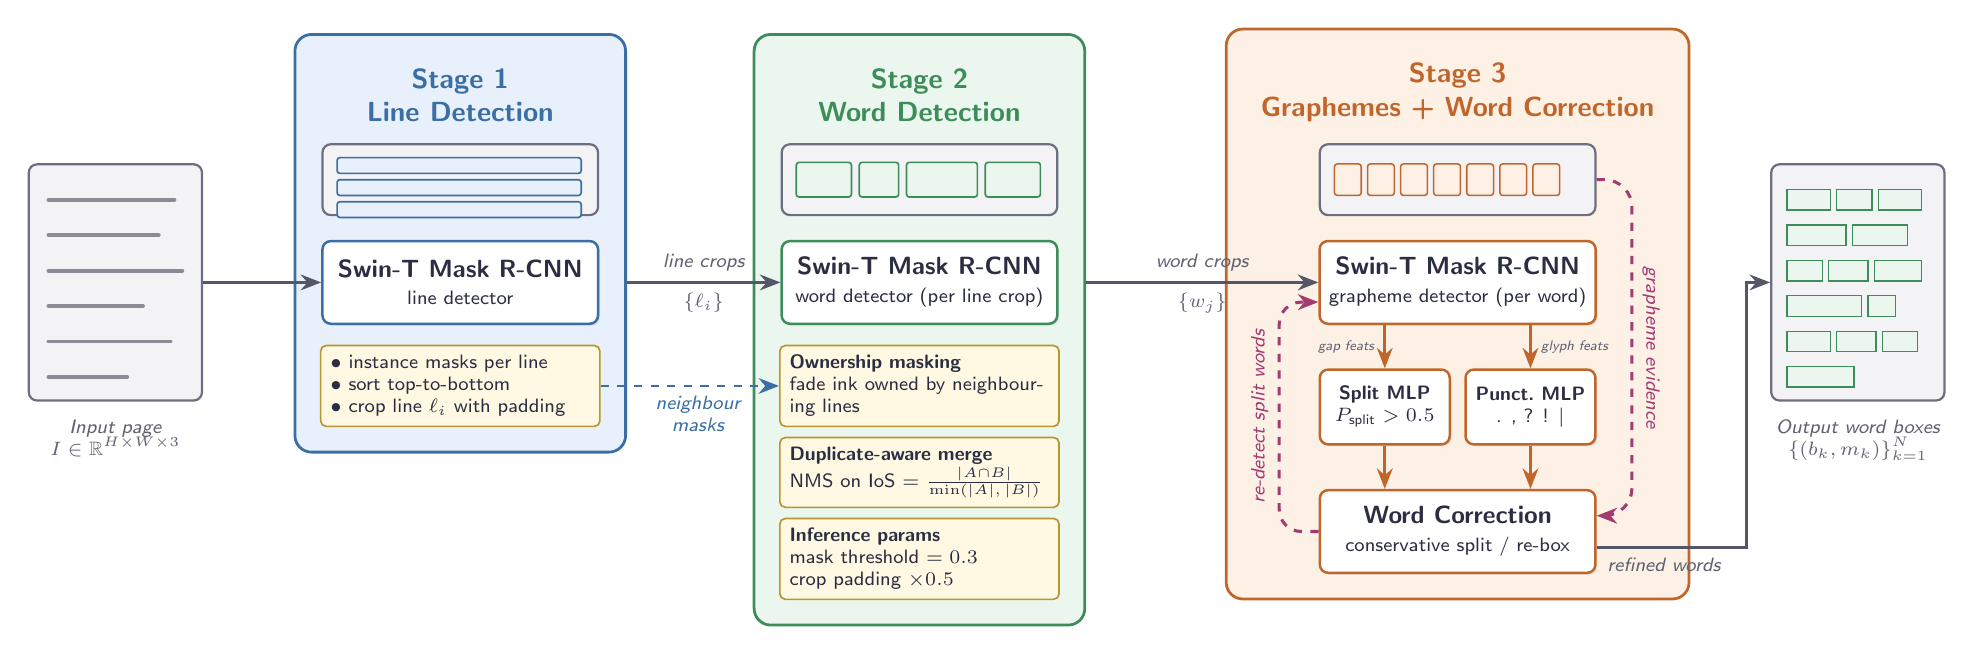
\begin{tikzpicture}[
  font=\sffamily\small, text=ink,
  >={Stealth[length=2.6mm,width=2mm]},
  flow/.style={->, line width=1.1pt, draw=ink!80},
  stage/.style={draw=#1, line width=1pt, rounded corners=6pt, inner sep=9pt},
  model/.style={draw=#1, fill=white, line width=0.9pt, rounded corners=3pt,
                minimum width=3.5cm, minimum height=1.05cm, align=center,
                drop shadow={shadow xshift=0.7pt, shadow yshift=-0.7pt, fill=black!18}},
  trk/.style={draw=trickD, fill=trick, line width=0.6pt, rounded corners=2pt,
              minimum width=3.5cm, align=left, font=\sffamily\scriptsize,
              inner sep=3.5pt, text width=3.3cm},
  head/.style={font=\sffamily\bfseries, text=#1, align=center},
  io/.style={draw=ioD, fill=ioF, line width=0.8pt, rounded corners=3pt, align=center},
  lbl/.style={font=\sffamily\scriptsize\itshape, text=ink!75, align=center},
]

% INPUT PAGE
\node[io, minimum width=2.2cm, minimum height=3.0cm] (page) at (0,0) {};
\foreach \y/\w in {1.05/1.6, 0.6/1.4, 0.15/1.7, -0.3/1.2, -0.75/1.55, -1.2/1.0}{
  \draw[ink!55, line width=1.4pt, line cap=round]
    ($(page.center)+(-0.85,\y)$) -- ++(\w,0);
}
\node[lbl, below=3pt of page] (pagelbl) {Input page\\$I \in \mathbb{R}^{H\times W\times 3}$};

% STAGE 1
\node[model=sOneD, right=1.5cm of page] (lineDet)
  {\textbf{Swin-T Mask R-CNN}\\[-1pt]{\scriptsize line detector}};
\node[trk, below=0.25cm of lineDet] (l1)
  {$\bullet$ instance masks per line\\$\bullet$ sort top-to-bottom\\$\bullet$ crop line $\ell_i$ with padding};
\node[io, above=0.3cm of lineDet, minimum width=3.5cm, minimum height=0.9cm] (lineCrops) {};
\foreach \k in {0,1,2}{
  \draw[sOneD, fill=sOneF, line width=0.6pt, rounded corners=1pt]
    ($(lineCrops.west)+(0.2,0.28-\k*0.28)$) rectangle ++(3.1,-0.2);
}
\node[head=sOneD, above=0.15cm of lineCrops] (h1) {Stage 1\\Line Detection};
\begin{scope}[on background layer]
  \node[stage=sOneD, fill=sOneF, fit=(h1)(lineCrops)(lineDet)(l1)] (S1) {};
\end{scope}

% STAGE 2
\node[model=sTwoD, right=2.3cm of lineDet] (wordDet)
  {\textbf{Swin-T Mask R-CNN}\\[-1pt]{\scriptsize word detector (per line crop)}};
\node[trk, below=0.25cm of wordDet] (w1)
  {\textbf{Ownership masking}\\fade ink owned by neighbouring lines};
\node[trk, below=0.12cm of w1] (w2)
  {\textbf{Duplicate-aware merge}\\NMS on IoS $=\frac{|A\cap B|}{\min(|A|,\,|B|)}$};
\node[trk, below=0.12cm of w2] (w3)
  {\textbf{Inference params}\\mask threshold $=0.3$\\crop padding $\times 0.5$};
\node[io, above=0.3cm of wordDet, minimum width=3.5cm, minimum height=0.9cm] (wordGly) {};
\foreach \x/\w in {0.2/0.7, 1.0/0.5, 1.6/0.9, 2.6/0.7}{
  \draw[sTwoD, fill=sTwoF, line width=0.6pt, rounded corners=1pt]
    ($(wordGly.west)+(\x,0.22)$) rectangle ++(\w,-0.44);
}
\node[head=sTwoD, above=0.15cm of wordGly] (h2) {Stage 2\\Word Detection};
\begin{scope}[on background layer]
  \node[stage=sTwoD, fill=sTwoF, fit=(h2)(wordGly)(wordDet)(w3)] (S2) {};
\end{scope}

% STAGE 3
\node[model=sThrD, right=3.3cm of wordDet] (grDet)
  {\textbf{Swin-T Mask R-CNN}\\[-1pt]{\scriptsize grapheme detector (per word)}};
\node[io, above=0.3cm of grDet, minimum width=3.5cm, minimum height=0.9cm] (grGly) {};
\foreach \x in {0.2,0.62,1.04,1.46,1.88,2.30,2.72}{
  \draw[sThrD, fill=sThrF, line width=0.55pt, rounded corners=1pt]
    ($(grGly.west)+(\x,0.2)$) rectangle ++(0.34,-0.4);
}
\node[head=sThrD, above=0.15cm of grGly]
  (h3) {Stage 3\\Graphemes + Word Correction};

\node[model=sThrD, below=0.55cm of grDet, minimum width=1.65cm, minimum height=0.95cm,
      xshift=-0.925cm, font=\sffamily\scriptsize] (splitC)
  {\textbf{Split MLP}\\$P_{\text{split}}>0.5$};
\node[model=sThrD, below=0.55cm of grDet, minimum width=1.65cm, minimum height=0.95cm,
      xshift=0.925cm, font=\sffamily\scriptsize] (punctC)
  {\textbf{Punct.\ MLP}\\. , ? ! $\mid$};
\node[model=sThrD, below=0.55cm of $(splitC.south)!0.5!(punctC.south)$,
      font=\sffamily\small] (corr)
  {\textbf{Word Correction}\\[-1pt]{\scriptsize conservative split / re-box}};

\draw[flow, draw=sThrD] (grDet.south -| splitC) -- node[lbl, left, font=\sffamily\tiny\itshape]{gap feats} (splitC.north);
\draw[flow, draw=sThrD] (grDet.south -| punctC) -- node[lbl, right, font=\sffamily\tiny\itshape]{glyph feats} (punctC.north);
\draw[flow, draw=sThrD] (splitC.south) -- (splitC.south |- corr.north);
\draw[flow, draw=sThrD] (punctC.south) -- (punctC.south |- corr.north);

\coordinate (fbL) at ($(grDet.west)+(-0.85,0)$);
\coordinate (fbR) at ($(grGly.east)+(0.7,0)$);
\begin{scope}[on background layer]
  \node[stage=sThrD, fill=sThrF, fit=(h3)(grGly)(grDet)(corr)(splitC)(punctC)(fbL)(fbR)] (S3) {};
\end{scope}

% OUTPUT
\node[io, minimum width=2.2cm, minimum height=3.0cm, right=2.2cm of grDet] (out) {};
\foreach \y/\x/\w in {
   1.05/-0.9/0.55,  1.05/-0.27/0.45,  1.05/0.26/0.55,
   0.60/-0.9/0.75,  0.60/-0.07/0.70,
   0.15/-0.9/0.45,  0.15/-0.37/0.50,  0.15/0.21/0.60,
  -0.30/-0.9/0.95,  -0.30/0.13/0.35,
  -0.75/-0.9/0.55,  -0.75/-0.27/0.50, -0.75/0.31/0.45,
  -1.20/-0.9/0.85}{
  \draw[sTwoD, fill=sTwoF, line width=0.5pt]
    ($(out.center)+(\x,\y+0.13)$) rectangle ++(\w,-0.26);
}
\node[lbl, below=3pt of out] {Output word boxes\\$\{(b_k, m_k)\}_{k=1}^{N}$};

% MAIN FLOW ARROWS
\draw[flow] (page.east) -- (lineDet.west);
\draw[flow] (S1.east |- lineDet) -- node[lbl, above]{line crops} node[lbl, below]{$\{\ell_i\}$} (wordDet.west);
\draw[flow] (S2.east |- wordDet) -- node[lbl, above]{word crops} node[lbl, below]{$\{w_j\}$} (grDet.west);
\draw[flow] ($(corr.east)+(0,-0.2)$) -- node[lbl, below, pos=0.45]{refined words} ++(1.9,0) |- (out.west);

% CONTEXT
\draw[->, dashed, line width=0.8pt, draw=sOneD]
  (l1.east) to[out=0,in=180] node[lbl, below, pos=0.55, text=sOneD]{neighbour\\masks} (w1.west);

% FEEDBACK LOOPS
\draw[->, line width=1.1pt, draw=fb, dashed, rounded corners=8pt]
  (corr.west) -- ++(-0.5,0) |- node[pos=0.25, lbl, text=fb, sloped, above]{re-detect split words} ($(grDet.west)+(0,-0.25)$);
\draw[->, line width=1.1pt, draw=fb, dashed, rounded corners=10pt]
  (grGly.east) -- ++(0.45,0) |- node[pos=0.25, lbl, text=fb, sloped, above]{grapheme evidence} ($(corr.east)+(0,0.2)$);

\end{tikzpicture}%
}% end resizebox
\vspace{-12pt}
\caption{Unified Line $\rightarrow$ Word $\rightarrow$ Grapheme Cascade Architecture. Input page flows left-to-right through three Swin-T Mask R-CNN stages. Stage 1 detects line polygons; Stage 2 detects words within line crops, applying three inference tricks (shown in yellow). Stage 3 detects graphemes and uses them to correct word boundaries via two MLPs (split and punctuation), with feedback loops (magenta dashed) showing grapheme evidence flowing back and corrected word locations re-entering the grapheme detector.}
\label{fig:architecture}
\end{figure}

\section*{9. Future Iterations and Roadmap}

The oracle analysis in Section 6 points to four concrete gaps and one deferred architectural change; this roadmap orders them by expected effort and payoff.

\textbf{1. Unified Single-Weight Checkpoint (near-term).} Today the engine runs three independent checkpoints (line, word, grapheme). The planned \texttt{composite/} model shares a single backbone across a line head, a word head, and a grapheme head, cutting total parameters by roughly 42\% relative to the current 144M three-checkpoint total and collapsing the cascade into one forward pass per page instead of one per stage. Training is estimated at about one GPU-week, using cascade-aware sampling so that the shared backbone sees the same overlapping-crop and ownership-masking conditions it will face at inference. The engine itself is model-agnostic and requires no changes to run against \texttt{composite/} once trained.

\textbf{2. Dedicated Punctuation Detector (near-term).} The current punctuation classifier is weak (AUC 0.83, only 651 positive marks out of roughly 15{,}600 candidates on dev, a heavily imbalanced problem for a generic MLP). Oracle analysis shows perfect punctuation handling alone is worth +0.05 F1, of which the current classifier captures only +0.003. A small detector trained specifically on synthetic punctuation marks, rather than a classifier bolted onto grapheme-run features, is the highest-value near-term fix.

\textbf{3. Selective Grapheme Inference (near-term, speed).} Running the grapheme model on every word triples per-page runtime (0.57 to 1.62\,s/page). Most words never need grapheme evidence because they are already correctly segmented after Benchmark 1. Restricting the grapheme pass to words flagged as likely merges by the existing word-model confidence and simple heuristics should avoid 60--70\% of grapheme inference calls, with an expected runtime of roughly 0.9\,s/page and minimal F1 loss.

\textbf{4. Improved Split Geometry (medium-term).} Oracle analysis shows +0.05 F1 remains in split-word box quality alone: correct splits placed with ground-truth-quality boxes reach split F1 0.905 on dev, against 0.851 with the current box geometry. Separately, 104 merged words on test have no grapheme gap at the true boundary at all, capping split recall at the candidate-generation stage regardless of classifier quality. A dedicated box-refinement head trained specifically for split-word geometry addresses the first; better split-candidate generation addresses the second.

\textbf{5. Cascade-Aware Data Augmentation (medium-term).} The grapheme model is trained independently of line/word context, so it never sees the overlapping-crop artifacts, ownership-masking fades, or duplicate-merge boundaries that the deployed cascade actually produces. Synthetic training data that reproduces these realistic line-overlap and crop-boundary patterns should improve how well ownership masking and merge handling generalize beyond the current dev/test split.

\textbf{6. Extension to Multi-Line Words (future).} The pipeline currently assumes every word fits inside a single line's crop, which holds for the vast majority of Bangla handwriting. Curved or heavily slanted lines could occasionally split a word across two line detections. An optional inter-line word-linking step in post-processing, triggered only when a word's box is truncated at a line boundary, would close this edge case without affecting the common path.

\section*{Artifacts}
\begin{itemize}
  \item \textbf{Code:} \texttt{unified\_cascade/}. \texttt{engine.py} is the cascade and tricks;
        \texttt{gaps.py}, \texttt{v3.py} and \texttt{punct.py} are the grapheme and punctuation
        editors; \texttt{bench.py} is the benchmark.
  \item \textbf{Every statistic:} \texttt{unified\_cascade/results/all\_stats.json} (all 11 runs,
        per-page counts, CV/oracle tables). Regenerate it with
        \texttt{python -m unified\_cascade.collect\_stats}.
  \item \textbf{Narrative log:} \texttt{unified\_cascade/RESULTS.md}.
  \item \textbf{Plan and literature:} \texttt{docs/cascade\_clever\_inference\_plan.md}.
\end{itemize}

\end{document}
